\documentclass[sigconf]{acmart}
\bibliographystyle{ACM-Reference-Format}
\usepackage{graphicx}
\usepackage{xurl}
\usepackage{float}
\usepackage{listings}

\lstset{
    basicstyle=\ttfamily\small, % Monospaced font
    breaklines=true,            % Automatically break long lines
    breakatwhitespace=true,     % Break lines at whitespace when possible
    frame=none,                 % No borders around the code block
    tabsize=4,                  % Set tab size
    xleftmargin=2em,            % Indent the block
    columns=fullflexible        % Adjust spacing for alignment
}

\title{Software Dependability Project Report}
\author{Aouni Wrocklage}\author{Janna Piontek}\author{Luka Nola}
\affiliation{%
  \url{https://github.com/orgs/Erasmus-In-Salerno/repositories}
}
\date{January 2025}
\renewcommand\footnotetextcopyrightpermission[1]{}
\settopmatter{printacmref=false}

\begin{document}

\maketitle
\pagestyle{plain}


\section{Introduction}

Why did we choose this project?
We chose \href{https://commons.apache.org/proper/commons-dbutils/}{Apache Commons dbUtils} for our Software Dependability course because it offers several advantages for a thorough security analysis. First, its \textbf{manageable size} makes it an ideal candidate for an in-depth examination without the complexity of larger frameworks. This allows us to focus on key components and security-related aspects without getting overwhelmed by an extensive codebase.

Additionally, although dbUtils is not part of Spring itself, it is commonly used in \textbf{Spring applications} to simplify complex JDBC (Java Database Connectivity) operations. This makes it highly relevant in real-world use cases, particularly in terms of securing database interactions in Spring environments. By analyzing dbUtils, we can gain valuable insights into its role within Spring-based applications and identify potential security concerns tied to database access.

A major factor in our decision is the emphasis of dbUtils on \textbf{resource management and security}. By abstracting JDBC operations, developers can avoid common issues, such as resource leaks and unclosed connections, which are often sources of security vulnerabilities. This makes it an excellent project for evaluating how well it handles these risks.

Finally, as part of the \textbf{Apache Commons project}, dbUtils benefits from strong community support and comprehensive documentation. This facilitates our ability to conduct a thorough security audit while assessing how well it adheres to security best practices over time.

In summary, we selected dbUtils because it strikes a balance between relevance, simplicity, and real-world security implications, particularly in the context of database operations within Spring applications.


\section{SonarCloud Analysis}

\begin{figure}[H]
    \centering
    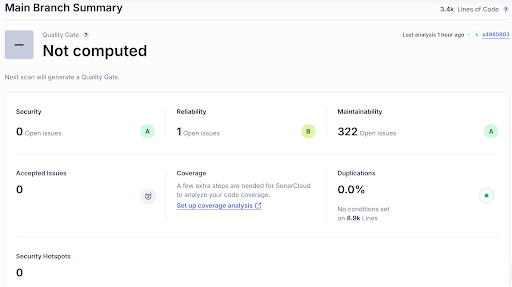
\includegraphics[width=1\linewidth]{images/sonarcloud.png}
    \caption{SonarCloud analysis}
\end{figure}

Analyzing the main branch of commons-dbutils with SonarCloud, one reliability issue and 322 maintainability code smells were found. The maintainability issues are separated into 239 low-severity issues, 56 medium-severity issues, and 27 high-severity issues, the latter representing the issues we will focus on. 
16 of the high-severity issues relate to JUnit tests and are based on the rule 'tests should include assertions', therefore requesting to add at least one assertion to the test case. Most of these issues relate to the DBUtilsTest class (src/test/java/org/apache/commons/dbutils/DbUtilsTest.java). Resolving them is marked to contribute to the clean code principle of adaptability. 
Another six of the high-severity issues violate the clean code principle of intentionality by leaving insufficiently documented empty methods in the code. To resolve the issue it is necessary to add a nested comment, to complete the implementation or to throw an UnsupportedOperationException.
Three more high-severity issues refer to the repeated duplication of string literals as error messages inside one class, instead of defining a constant for them. 
The last two high-severity issues relate to one method each, whose cognitive complexity is too high, meaning that the code is difficult to understand. While in general several different aspects contribute to the cognitive complexity of a method (\url{https://docs.codeclimate.com/docs/cognitive-complexity}), the criticized methods mainly use multiple conditionals and loops nested inside each other. Solving the issues therefore requires a restructuring of the methods.

\textbf{Not fixed high-severity issues:}
\begin{itemize}
    \item \url{https://sonarcloud.io/project/issues?open=AZKLhIh2Sh2-aRAfcuMl&id=Erasmus-In-Salerno_commons-dbutils}
    \item \url{https://sonarcloud.io/project/issues?open=AZKLhIh2Sh2-aRAfcuMm&id=Erasmus-In-Salerno_commons-dbutils}
    \item \url{https://sonarcloud.io/project/issues?open=AZKLhIh2Sh2-aRAfcuMn&id=Erasmus-In-Salerno_commons-dbutils}
\end{itemize}

These three issues weren’t fixed because the underlying rule “tests should include at least one assertion” did not really apply to the specific code sections. All three issues are related to JUnit tests calling an overloaded method, that closes a connection, result set or a statement respectively. They test null handling, but as the method is supposed to do nothing when given a null parameter, the only assertion that could be made, is that no exception is thrown. As JUnit tests fail by default when an exception is thrown, adding an assertion would be unnecessary.

\begin{itemize}
    \item \url{https://sonarcloud.io/project/issues?open=AZKLhIh2Sh2-aRAfcuMo&id=Erasmus-In-Salerno_commons-dbutils}
    \item \url{https://sonarcloud.io/project/issues?open=AZKLhIh2Sh2-aRAfcuMp&id=Erasmus-In-Salerno_commons-dbutils}
    \item \url{https://sonarcloud.io/project/issues?open=AZKLhIh2Sh2-aRAfcuMq&id=Erasmus-In-Salerno_commons-dbutils}
    \item \url{https://sonarcloud.io/project/issues?open=AZKLhIh2Sh2-aRAfcuMr&id=Erasmus-In-Salerno_commons-dbutils}
    \item \url{https://sonarcloud.io/project/issues?open=AZKLhIh2Sh2-aRAfcuMs&id=Erasmus-In-Salerno_commons-dbutils}
    \item \url{https://sonarcloud.io/project/issues?open=AZKLhIh2Sh2-aRAfcuMt&id=Erasmus-In-Salerno_commons-dbutils}
\end{itemize}

The same applies to these six issues, all of which refer to tests without assertions of the same method. This method (closeQuietly()) calls the close method that was tested in the test cases mentioned above. The only difference between the two methods is that SQL exceptions are ignored. Therefore, calling the closeQuietly method with null has the same effect as calling the close method with null, meaning that the justification why the corresponding (3) issues were not fixed is the same as above. The other three issues test whether SQL exceptions are properly ignored. If everything works as expected, no exception reaches the test method, so the test succeeds. If something goes wrong and an exception is thrown, the test will fail anyway, so again, no assertions are needed.

\section{Docker}
Since the project is a database utility library there was no real way of building, dockerizing and presenting the image without some sort of application that uses it as a dependency. For this reason, a web app was created. The web app, built using Spring Boot, consists of a simple UI that allows the user to see all the animals in the database, to add a new one, or to delete one by id. The database connection and queries are managed with our fork of the DbUtils library. For the detailed explanations on how to run, build and compose the app, check out the project \href{https://github.com/Erasmus-In-Salerno/dbUtils-webapp}{README.md}. The image we are building contains this app while we compose it together with the postgres database it needs to be connected to.

\subsection*{Building the Docker Image}
In the case of Spring Boot, building a Docker image is trivial; by running the command:
\begin{verbatim}
    $ mvn spring-boot:build-image -DskipTests
\end{verbatim}

\texttt{-DskipTests} was used because the tests have not been set up on this project so there was no need to run them. 

This created the image named \texttt{dbutils-webapp:latest}. That was tagged and pushed to DockerHub using the commands:

\begin{lstlisting}
$ docker tag dbutils-webapp:latest lukanola/dbutils-webapp:latest
$ docker push lukanola/dbutils-webapp:latest
\end{lstlisting}

and is available on this link: \url{https://hub.docker.com/repository/docker/lukanola/dbutils-webapp/}. This image is now ready for orchestration.

An alternative approach would be to write the \texttt{Dockerfile} similar to Figure 2 which would start with a \texttt{maven} base to build the package and after that using the \texttt{openjdk} package as a base, would run the built \texttt{jar}.

\begin{figure}
    \centering
    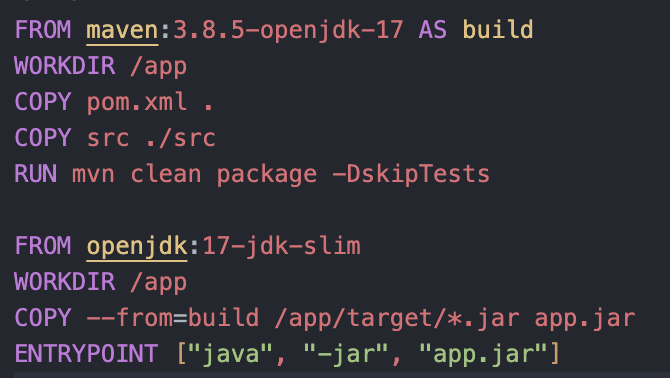
\includegraphics[width=1\linewidth]{images/docker.png}
    \caption{Dockerfile example}
\end{figure}

\subsection*{Composing the Containers}
Since the app requires a database connection to function and demonstrate the DbUtils library we need to orchestrate two containers, one containing the app itself and another containing the postgres database. We can do this by creating a \texttt{docker-compose.yml} file and defining two services - db and app. 

The \textbf{db container} runs from the public image \texttt{postgres:latest} while exposing the correct port and setting the correct environment variables.

The \textbf{app container} runs from the dbutils-webapp we built and while exposing the port 8080 and setting the environment variables. Since we don't want the app to run before the database is running in the container we set that the app container \textbf{depends} on the db container.

Now the project is runnable and deployable on any machine (that has Docker installed) and can be managed by a service for managing containerized apps such as Kubernetes.

\section{Code coverage analysis with Jacoco}

\begin{figure}[H]
    \centering
    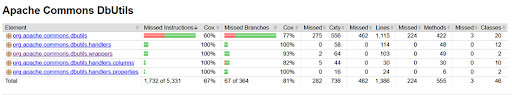
\includegraphics[width=1\linewidth]{images/jacoco1.png}
    \caption{Overview of JaCoCo Results}
\end{figure}

When looking more closely at the result you see that the missed things from the tests are nearly all concentrated in the base package, where also the biggest part of the logic lies.

\begin{figure}[H]
    \centering
    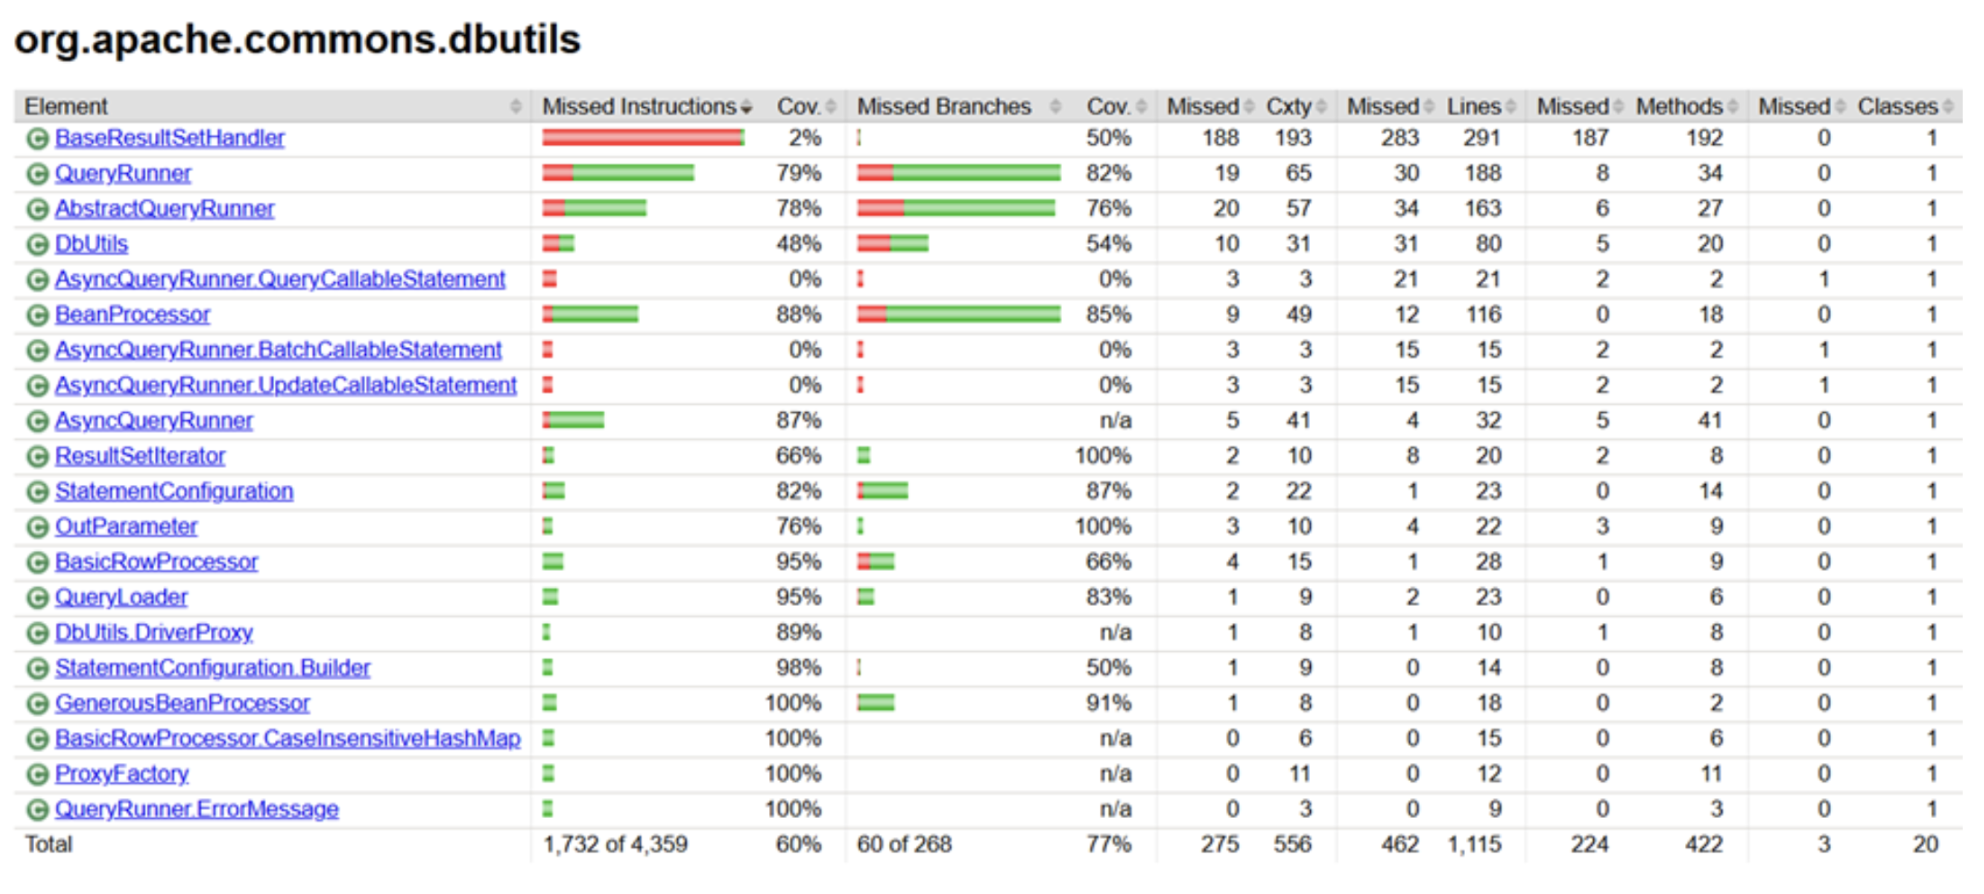
\includegraphics[width=1\linewidth]{images/jacoco2.png}
    \caption{JaCoCo overview for the package "org.apache.commons.dbUtils"}
\end{figure}

A closer analysis of the results highlights significant disparities in test coverage among the classes. Most classes exhibit close to 80\% coverage, yet the \texttt{BaseResultSetHandler} stands out negatively, with an abysmal 2\% instruction coverage, 2.5\% complexity coverage, and just 3\% line coverage. This class, the largest in the package, serves as a utility for interacting with \texttt{ResultSet} objects by providing pre-defined methods to streamline database operations and minimize boilerplate code while maintaining flexibility for various conversion needs.

While the library as a whole demonstrates a generally acceptable test coverage level, the glaring coverage gap in the \\
\texttt{BaseResultSetHandler} is a critical weakness, given the extensive logic and code it contains. Addressing this shortfall would significantly improve the library's reliability and robustness.

Beyond the \texttt{BaseResultSetHandler}, the \texttt{DbUtils} class also demands attention, with only 48\% test coverage. Additionally, the \texttt{QueryRunner} and \texttt{AbstractQueryRunner} classes, both falling just below the 80\% threshold, further underline the need for more comprehensive testing. These classes have been identified as priorities for additional test case generation to enhance overall code quality and coverage metrics.

\subsection*{Brief Description of the Worst Tested Classes}

In the following section, the classes that do not have good test coverage are described briefly.

\subsubsection*{\textbf{BaseResultSetHandler}}

The \texttt{BaseResultSetHandler} is an abstract class designed to simplify the process of converting SQL \texttt{ResultSet} objects into various target types, such as lists, maps, or custom objects. It serves as a base class for implementing reusable result set handlers. The class provides a range of standard utility methods for handling \texttt{ResultSet}s (e.g., \texttt{absolute}, \texttt{beforeFirst}, \texttt{deleteRow}, \texttt{getObject}, and many more). These methods are intended to make working with \texttt{ResultSet} easier and to eliminate repetitive code when interacting with SQL query results.

\subsubsection*{\textbf{DbUtils}}

\texttt{DbUtils} is a utility class that provides a simple set of helper functions for working with JDBC (Java Database Connectivity). This class is designed to make handling database resources easier and to address common issues, such as properly closing connections, statements, and result sets.

\subsubsection*{\textbf{QueryRunner}}

The \texttt{QueryRunner} class simplifies executing SQL queries and updates in Java applications. It provides a high-level API for managing database interactions, focusing on reducing repetitive boilerplate code required when working with JDBC directly. Supports SQL queries (\texttt{SELECT}), updates (\texttt{INSERT}, \texttt{UPDATE}, \texttt{DELETE}), and batch operations. Integrates with pluggable \texttt{ResultSetHandler} implementations to process and map \texttt{ResultSet} data into Java objects.

\subsubsection*{\textbf{AbstractQueryRunner}}

The base class for the described \\ \texttt{QueryRunner} above.

\section{Mutation testing with Pitest}
We are using Pitest to evaluate the quality of the existing tests in the “\textbf{Apache Commons DBUtils}” repository. For executing the pitest-analysis, here and in future applications, the command “mvn org.pitest:pitest-maven:mutationCoverage” was used to evaluate the mutation coverage with pitest.

\begin{figure}[H]
    \centering
    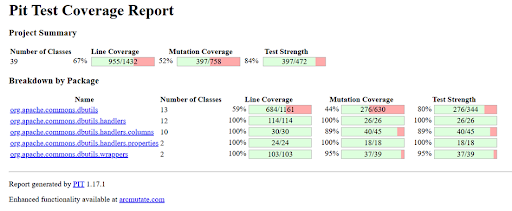
\includegraphics[width=1\linewidth]{images/pitest1.png}
    \caption{Pitest Analysis Overview}

\end{figure}

While the \textbf{line coverage} was previously analyzed in the JaCoCo report, the primary focus of the Pitest analysis lies in the \textbf{mutation coverage} and \textbf{test strength}. Although the overall Test Strength of 84\% is relatively high, the Mutation Coverage of 52\% is noticeably lower.

\begin{figure}[H]
    \centering
    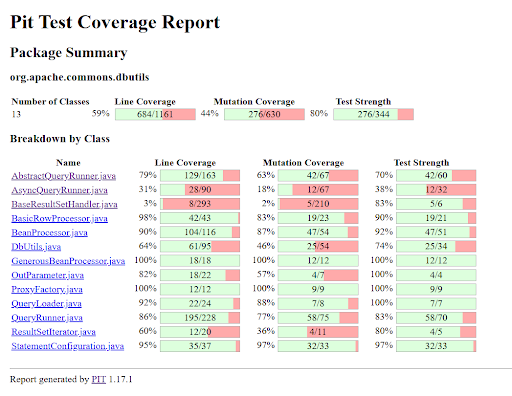
\includegraphics[width=1\linewidth]{images/pitest2.png}
    \caption{“org.apache.commons.dbutils” Package Pit Test Overview}
\end{figure}

A low mutation score is often related to low line coverage because, although mutations are applied to all lines of code, only those mutations in lines executed by tests can potentially be killed. For untested lines of code, any mutations will inevitably survive, as there are no tests to evaluate them.

\vspace{0.5cm}

As seen in Figure 6, this is particularly evident in the classes \texttt{\textbf{AsyncQueryRunner}} and \texttt{\textbf{BaseResultSetHandler}}, as both have very low line coverage and, consequently, fail to achieve meaningful mutation coverage. To improve these metrics, it is essential to add tests for these classes.

\vspace{0.5cm}

The \texttt{\textbf{AsyncQueryRunner}} also stands out negatively in the analysis of “Test Strength": while all other classes achieve a test strength of over 70\%, this class reaches only 36\%. This indicates that the few existing tests neither sufficiently cover nor effectively evaluate this class.

These results clearly demonstrate that the critical and central class \texttt{AsyncQueryRunner} requires a more thorough examination, both in terms of test quantity, quality, and their ability to target and cover mutations effectively.

\section{Microbenchmark Performance Tests using JMH}

The \textbf{JMH} library was used to create microbenchmark performance tests for some of the most cumbersome classes and methods in the project. Those are:

\begin{itemize}
    \item \texttt{BasicRowProcessorBenchmark.java}
    \begin{itemize}
        \item \texttt{toArray}
        \item \texttt{toBean}
        \item \texttt{toBeanList}
    \end{itemize}
    \item \texttt{DbUtilsBenchmark.java}
    \begin{itemize}
        \item \texttt{close}
        \item \texttt{closeQuietly}
        \item \texttt{commitAndClose}
        \item \texttt{rollbackAndClose}
    \end{itemize}
    \item \texttt{QueryRunnerBenchmark.java}
    \begin{itemize}
        \item \texttt{query}
        \item \texttt{batch}
        \item \texttt{update}
    \end{itemize}
\end{itemize}


A new project, located in the root of the original library, was created to separate the dependencies and their effects on the result of the tests. The original library was added as a dependency of this new project.

\subsection*{Running the benchmark}
The benchmark can be run in the terminal with:

\begin{lstlisting}
mvn clean install in the root
mvn clean install in ./benchmarks and 
java -jar target/prova-1.0-SNAPSHOT.jar -rf json in ./benchmarks
\end{lstlisting}

\texttt{-XX:+EnableDynamicAgentLoading} can be added as an option to the last command to prevent the Mockito dynamic agent loading warnings.

\subsection*{Test Results}
The result of running these tests can be seen in the Figure 7 or in the \href{https://github.com/Erasmus-In-Salerno/commons-dbutils/blob/master/benchmark/jmh-result.json}{\texttt{jmh-result.json}}
included in the project.

\begin{figure}[H]
    \centering
    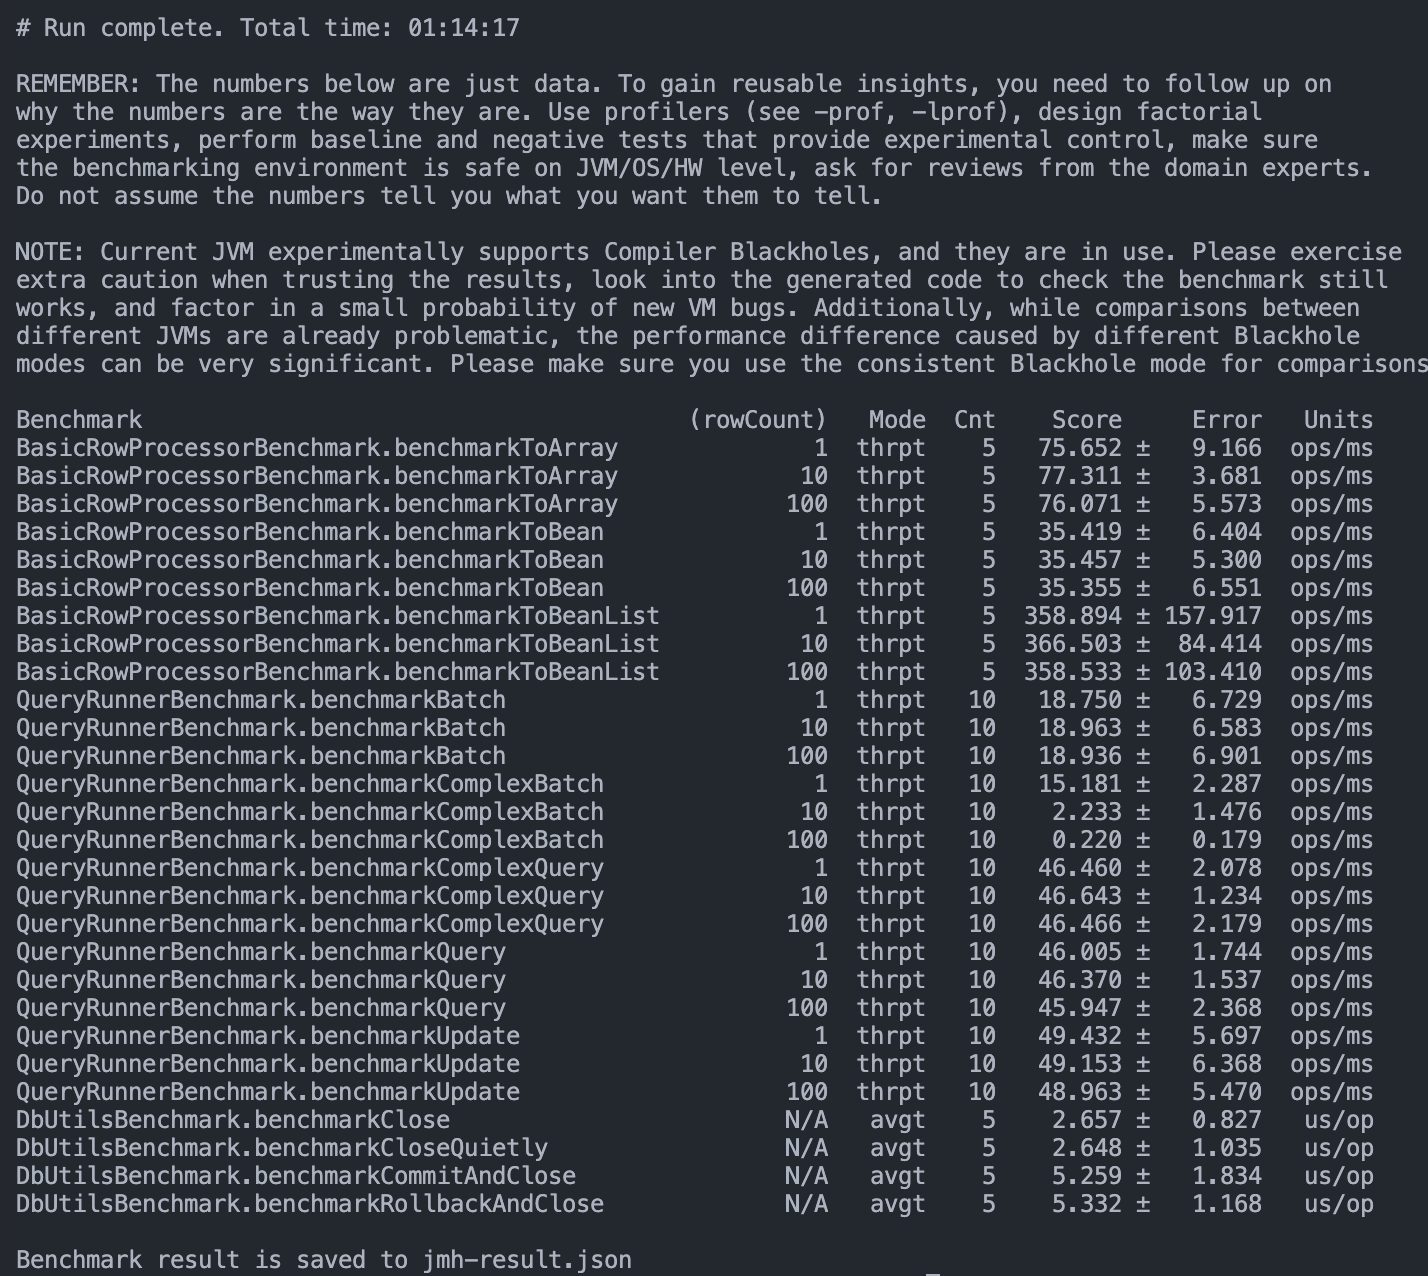
\includegraphics[width=1\linewidth]{images/jmh.png}
    \caption{JMH results}
\end{figure}

All of the results were expected. In this state, they represent the baseline for changes; meaning there should not be big differences when it comes to changing these methods in the future.

\subsection*{The Way the Test Was Conducted}

The tests are run in 5/10 iterations to reduce the effect of randomness and variance in the results. Also, 5/10 warmups are performed before the actual iterations to allow the system/JVM to stabilize, ensuring that any setup or transient state does not skew the final results.

The simplest are the tests for the \texttt{\textbf{DbUtils}} class. Each benchmark starts by opening a mock connection and closing it in the end. The chosen benchmark mode for these methods was \textbf{average time} since we want to benchmark the time it takes for the connection to close and commit/rollback to execute. Since \texttt{benchmarkCommitAndClose} and \texttt{benchmarkRollbackAndClose} both include the close call as well, it makes sense that the average time for them to execute is longer than just \texttt{benchmarkClose} and \texttt{benchmarkCloseQuietly}. We can notice that the difference in average execution time between the \texttt{close} and \texttt{closeQuietly} methods is negligible, being around 2.6 microseconds per operation. The same can be said about \texttt{commit} and \texttt{rollback} with those being around 5.25 microseconds per operation.

The chosen benchmark mode for \texttt{\textbf{BasicRowProcessor}} was\\ \textbf{throughput} because checking the amount of operations the system can run in a time frame tells us how the system performs under load and what the expected output is under \textbf{high load}. The tests consist of a setup that mocks a database connection and the data in the database that needs to be managed. In testing, we change the number of rows from 1 to 10 to 100 to better gauge the system performance under higher load. What we can see from the results is that the change in the number of rows doesn’t affect the results as much; perhaps a higher number would do so, but for the scope of the usage of this library, the performance differences are negligible. In terms of performance, \texttt{toBeanList} is generally more efficient when dealing with multiple rows because it processes the entire \texttt{ResultSet} in a single operation, reducing the overhead associated with multiple method calls. This aligns with the benchmarking results observed, where \texttt{toBeanList} has a significantly higher throughput than \texttt{toBean} and \texttt{toArray}.

Since the \texttt{\textbf{QueryRunner}} class deals with data and includes lots of connections that need to be tended to at the same time, \textbf{throughput} was the best benchmark mode. These benchmarks showed a lot of variations in the results and during warmup, so the number of iterations for both was increased to 10, which seems to have had a positive impact on the variance of the results. In the same way we changed the number of rows from 1 to 10 to 100 for the \texttt{BasicRowProcessor}, the same was done here with the parameters. The benchmarks all include mocking of the database connection and the data; however, some methods are tested twice. 
\\ The reason for this is to demonstrate how \textbf{costly and complex operations} affect the \textbf{throughput}. Between \texttt{benchmarkQuery} and \\ \texttt{benchmarkComplexQuery}, as well as \texttt{benchmarkBatch} and \\ \texttt{benchmarkComplexBatch}, we notice that the complexity of the method lowers the throughput, essentially making the execution slower (as expected).

\vspace{0.5cm}
It shows that the results of these benchmarks are as expected and now serve a purpose of being the baseline for future changes; allowing for easier detection of performance regressions and also helping validate performance improvements. Other than serving as a reference for changes, benchmarks such as these can help point out bottlenecks in the system, find issues before they pop up in usage, and much more.


\section{Automated test generation}
\subsection*{Randoop}

To identify poorly tested classes for generating additional test cases, the JaCoCo code coverage and PIT mutation testing results were analyzed. Based on this analysis, six classes were selected as priorities for further testing due to their low coverage or significant importance within the project. Even though having a high instruction coverage, the \texttt{BeanProcessor} was added because of its total number of missed instructions, which provided room for improvements. The chosen classes are:

\begin{itemize}
    \item \texttt{org.apache.commons.dbutils.BaseResultSetHandler}
    \item \texttt{org.apache.commons.dbutils.DbUtils}
    \item \texttt{org.apache.commons.dbutils.QueryRunner}
    \item \texttt{org.apache.commons.dbutils.AsyncQueryRunner}
    \item \texttt{org.apache.commons.dbutils.AbstractQueryRunner}
    \item \texttt{org.apache.commons.dbtils.BeanProcessor}
\end{itemize}

To generate test cases with Randoop, the following command was issued on project level in Windows 10 PowerShell:

\begin{lstlisting}
& 'C:\Program Files\Java\jdk-11.0.2\bin\java.exe' 
-classpath "..\randoop-4.3.3\randoop-all-4.3.3.jar;target\classes" 
randoop.main.Main gentests --classlist=..\PoorlyTestedClasses.txt --time-limit=600
\end{lstlisting}

As the project’s \texttt{pom.xml} Maven file declares the language and compilation level as 11, Java 11 is explicitly called to run Randoop to ensure compatibility with the project. The time-limit was set to 600, following the suggestion in the tool’s documentation (\href{https://randoop.github.io/randoop/manual/}{https://randoop.github.io/randoop/manual/}, accessed 8.12.2024) to multiply the default 100 by the number of tested classes.

Randoop generated a JUnit test suite of 9092 regression test cases divided into 19 test classes. Neither error-revealing nor invalid tests were generated. After moving the test files to the project’s test folder and adding the corresponding package declaration to the beginning of each file, the regression test suite ran successfully, as expected. Despite the high number of test cases and the length of each test file (approximately 35,000 lines of code), the test suite could be run reasonably fast.

\subsection*{JaCoCo}

\begin{figure}[H]
    \centering
    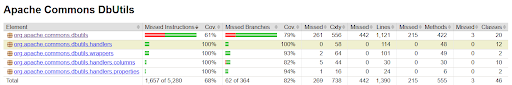
\includegraphics[width=1\linewidth]{images/randoop1.png}
    \caption{Overview of JaCoCo results}
\end{figure}

\begin{figure}[H]
    \centering
    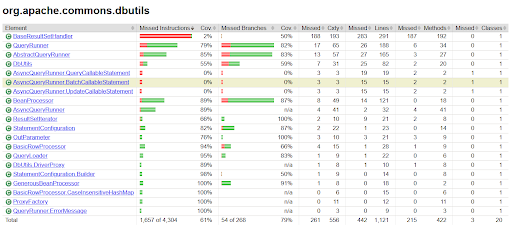
\includegraphics[width=1\linewidth]{images/randoop2.png}
    \caption{JaCoCo overview for the package "org.apache.commons.dbUtils"}
\end{figure}

\subsection*{Randoop-Generated Test Suite Results}

The with Randoop generated test suite significantly improved the test coverage of the \texttt{AbstractQueryRunner} and \texttt{DbUtils} classes and also provided better coverage results for the \texttt{AsyncQueryRunner} classes while it barely improved the \texttt{QueryRunner} class and did not improve the test coverage of the \texttt{BaseResultSetHandler} class at all.

There are multiple possible reasons for the results. As the randomly generated test cases do not take into account the already existing test cases that existed before using Randoop, it is more unlikely that test cases are generated, which cover prior untested code. This especially applies to larger classes which are already quite well tested. The \texttt{QueryRunner} class is such an example.

Differences in the results can also originate from the structure of the classes under test. As the \texttt{BaseResultSetHandler} is an abstract class, containing only protected and private methods, meant to be extended by the user of the \texttt{dbUtils} project, Randoop was not able to generate any test cases for it.

Afterall, Randoop is a tool based on random generation. If no randomness controlling seed is provided which stays the same, test generations will differ from each other, even if the code base stays unchanged, making it impossible to fully explain the results in detail.

\subsection*{Generation of Test Cases with GitHub Copilot}

While it makes sense to use Randoop on more classes, because in theory the tool is meant to be used on whole projects, we wanted to target the test generation with GitHub Copilot even more on still poorly tested classes. Therefore, the \texttt{BaseResultSetHandler}, \texttt{AsyncQueryRunner} (especially the inner classes), and \texttt{DbUtils} \\
classes were chosen as subjects for the test generation with GitHub Copilot, as they stick out with results below 75\% for line, instruction, and branch coverage and mutation coverage below 50\%.

\subsubsection*{\textbf{Test Generation for BaseResultSetHandler}}

GitHub Copilot Chat (hereafter just referred to as Copilot) was used as an integrated tool in IntelliJ Ultimate to generate more test cases for the prior very poorly tested (line coverage of 2\%) \texttt{BaseResultSetHandler} class. Copilot mainly used the \texttt{BaseResultSetHandler} (class under test) and the \texttt{BaseResultSetHandlerTest} classes to generate the test cases, but sometimes also used the \texttt{pom.xml} and the \texttt{BaseTestCase} class, which the \texttt{BaseResultSetHandlerTest} class extends, as resources.

After the initial prompt "generate test cases for the BaseResultSetHandler class," some fine-tuning was needed to generate proper test cases. As the \texttt{BaseResultSetHandler} is an abstract generic class, its test class needs to provide its own class which extends the \texttt{BaseResultSetHandler} and overwrites the \texttt{handle()} method. All other methods of the \texttt{BaseResultSetHandler} can only be called from inside the overwritten \texttt{handle()} method, because otherwise, the \texttt{ResultSet}, on which all methods work, is \texttt{null}. At first, Copilot did not understand this and tried to call all methods separately, which always caused \texttt{NullPointerExceptions}. Copilot was taught that each test method needs its own implementation of the \texttt{handle()} method, by providing it with an example improvement of a faulty test method.

Another issue was that Copilot generated test cases which used raw forms of the \texttt{BaseResultSetHandlerTest}, so all "Object" return results needed to be cast back to what they should resemble. Even though it worked, it is not a good way to do it, so Copilot was asked to change the prior generated test methods to use a specific type instead of \texttt{Object}.

When the generated test cases looked good and did not cause any problems anymore, Copilot was asked to generate test cases for all still untested methods. As the answer was interrupted because it became too long, the prompt was changed to "generate test methods for the next 20 still untested methods of the BaseResultSetHandler." This worked well several times after each other, each time resulting in an output of about 300 lines. A downside of generating test cases iteratively with Copilot was the increasing number of test methods which were already defined in the test class. Finally, "make sure not to generate test methods which are already defined in \texttt{BaseResultSetHandlerTest.java}" was added to the prompt to contain the problem, but it did not really improve the result. If an output included already existing methods, these few methods were deleted, while the rest was included in the test class. Other small variations of the prompt were tried until the line coverage (analyzed by IntelliJ) of the \texttt{BaseResultSetHandler} class was above 80\%.

In the process, almost 200 test methods were generated, spanning around 2650 lines of code. The quality of the tests was not analyzed. All tests passed, no errors were revealed.

\subsubsection*{\textbf{Test Generation for DbUtils}}

Compared to the \\ \texttt{BaseResultSetHandler}, \texttt{DbUtils} is much smaller and already better tested (line coverage around 50\%). Therefore, a more focused approach was needed. After highlighting some of the untested methods, the prompt "/tests write tests for the highlighted methods, that can be added to the tests in \#DbUtilsTest.java" was used to generate test cases for the methods. The command was repeated with another highlighted section of untested methods. In total, around 15 test methods were generated, improving the test coverage of the \texttt{DbUtils} class significantly.

\subsubsection*{\textbf{Test Generation for AsyncQueryRunner}}

The \\ \texttt{AsyncQueryRunner} itself already has a satisfactory amount of tests. However, its inner classes \texttt{BatchCallableStatement}, \\ \texttt{UpdateCallableStatement}, and \texttt{QueryCallableStatement} do not have any tests. Copilot was used to address this gap. Tests for the first two inner classes were not generated because both classes are marked as "Deprecated." For \texttt{QueryCallableStatement}, Copilot did generate a test, but the test did not work as Copilot had issues instantiating a correct object of type \\ \texttt{AsyncQueryRunner.QueryCallableStatement}. This issue had to be resolved manually.

This example highlights the limitations of Copilot for flawless test creation, particularly when dealing with more complex code structures, such as correctly instantiating objects with intricate dependencies or nested class designs.

\subsection*{Changes in code coverage with JaCoCo}

\begin{figure}[H]
    \centering
    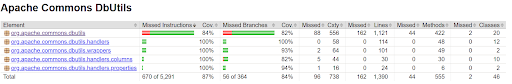
\includegraphics[width=1\linewidth]{images/jacoco3.png}
    \caption{Overview of JaCoCo results}
\end{figure}

\begin{figure}[H]
    \centering
    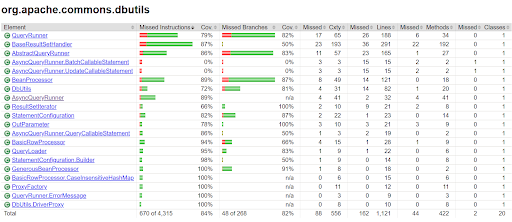
\includegraphics[width=1\linewidth]{images/jacoco4.png}
    \caption{JaCoCo Overview for the package org.apache.commons.dbUtils}
\end{figure}

The generation of test cases with Copilot significantly improved the instruction coverage of the classes \texttt{BaseResultSetHandler} (2\% → 87\%) and \texttt{DbUtils} (55\% → 72\%). As the generated tests did not reveal errors, they can be classified as regression tests. As these, they lower the risk of introducing bugs and unintended changes in method behavior, improving maintainability especially for the \texttt{BaseResultSetHandler}.

\subsection*{Comparison: Randoop - Github Copilot}
In comparison to the test generation with Randoop, the results show a clear superiority of Copilots test generation in terms of bringing test coverage close to the 80\% threshold. The generated tests could be seamlessly integrated into existing test files, opening the possibility to adapt them and change their order manually, which would not be possible in the code overhead Randoop produces for the coverage improvements. On the other hand the generation needed more manual interactions, making it a less automatic process and increasing the time needed for the improvements.

\begin{figure}[H]
    \centering
    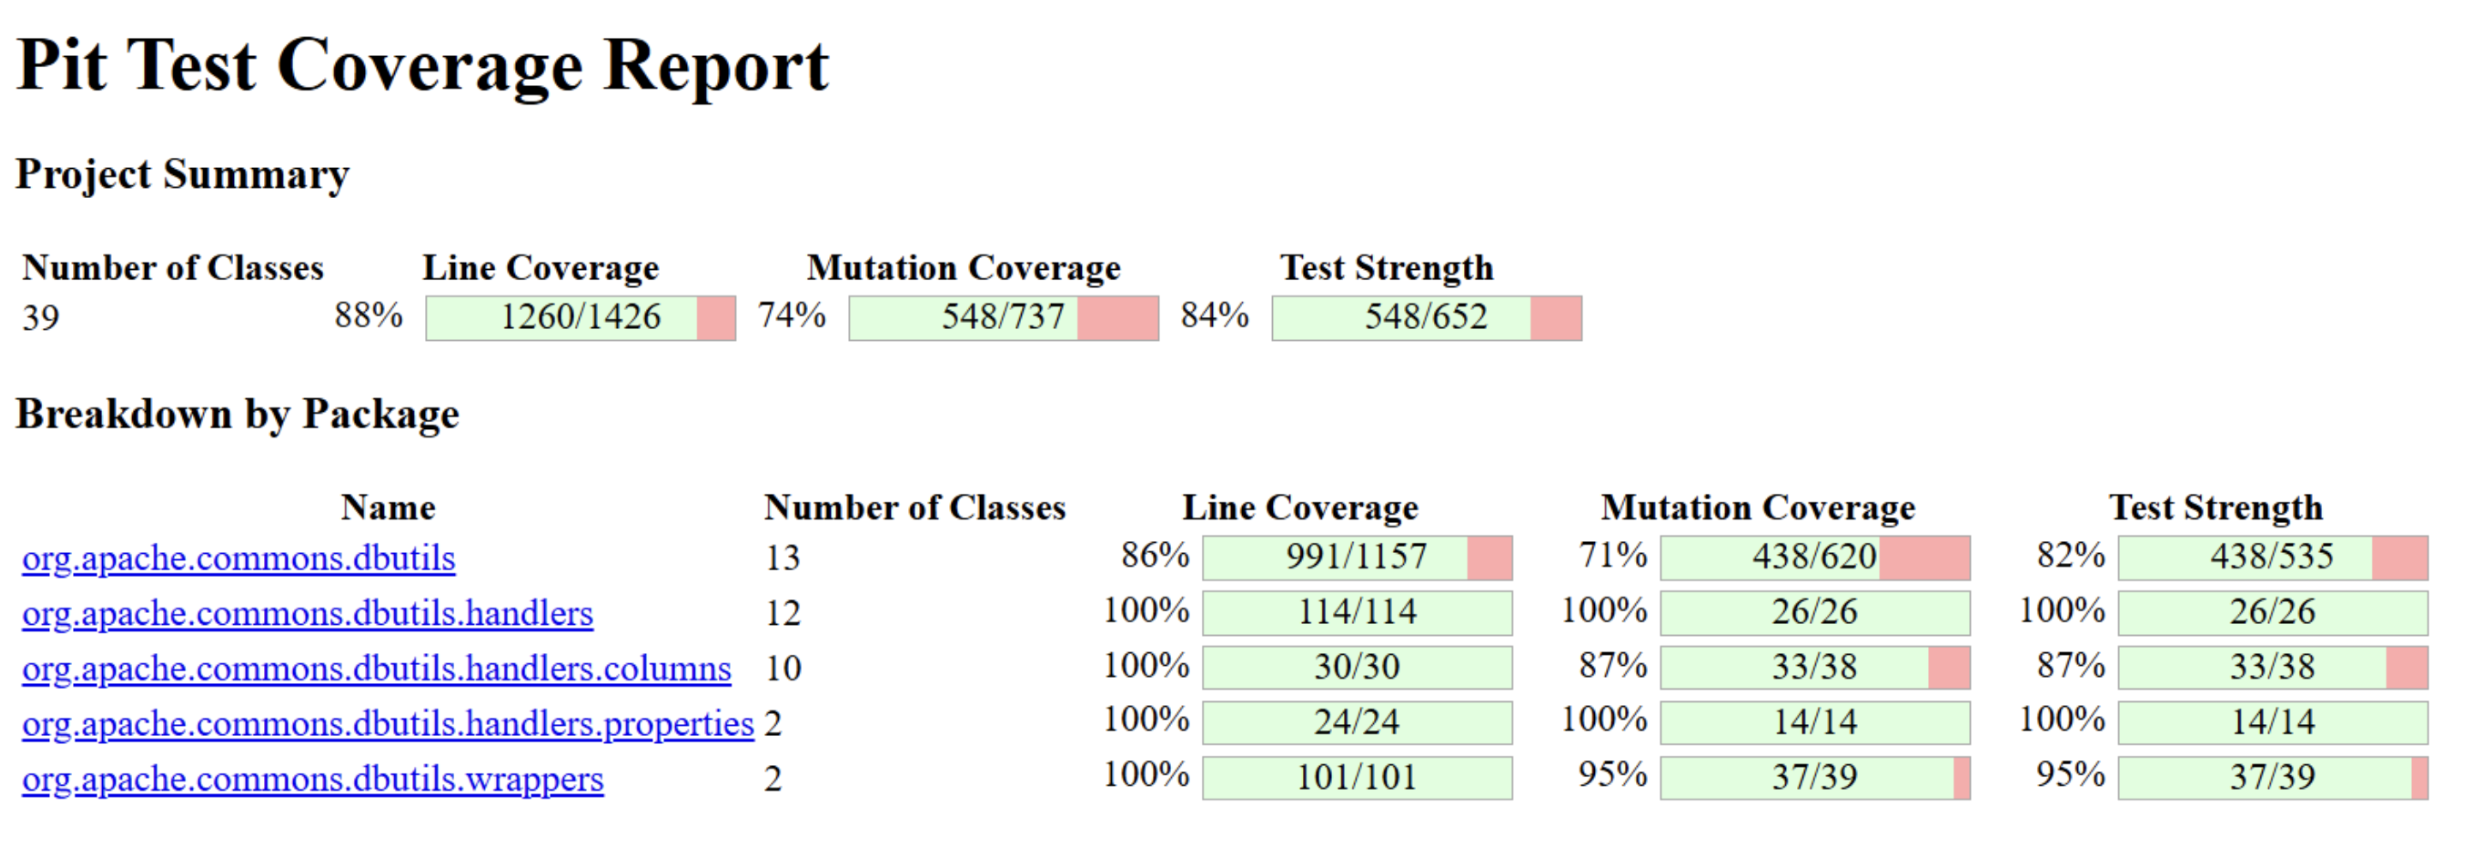
\includegraphics[width=1\linewidth]{images/pitest3.png}
    \caption{Pitest Analysis Overview}
\end{figure}

\subsection*{Changes in Mutation Coverage with Pitest}

As highlighted in the Pit Test analysis, the primary focus of this evaluation is on Mutation Coverage and Test Strength. Following the new test generation, the total number of tests included in the test strength calculation increased significantly, rising from 344 to 652—an improvement of nearly 90\%. Alongside the increase in test quantity, the test strength itself improved by 4 percentage points, reaching 84\%.

Similarly, mutation coverage, another critical metric in this analysis, experienced a notable increase from 44\% to 74\%. Overall, these results demonstrate that the generated tests have significantly enhanced the quality of testing within this library. However, a more detailed examination of the \texttt{dbUtils} base package is necessary to identify potential areas for further improvement and address any missed opportunities.

\begin{figure}[H]
    \centering
    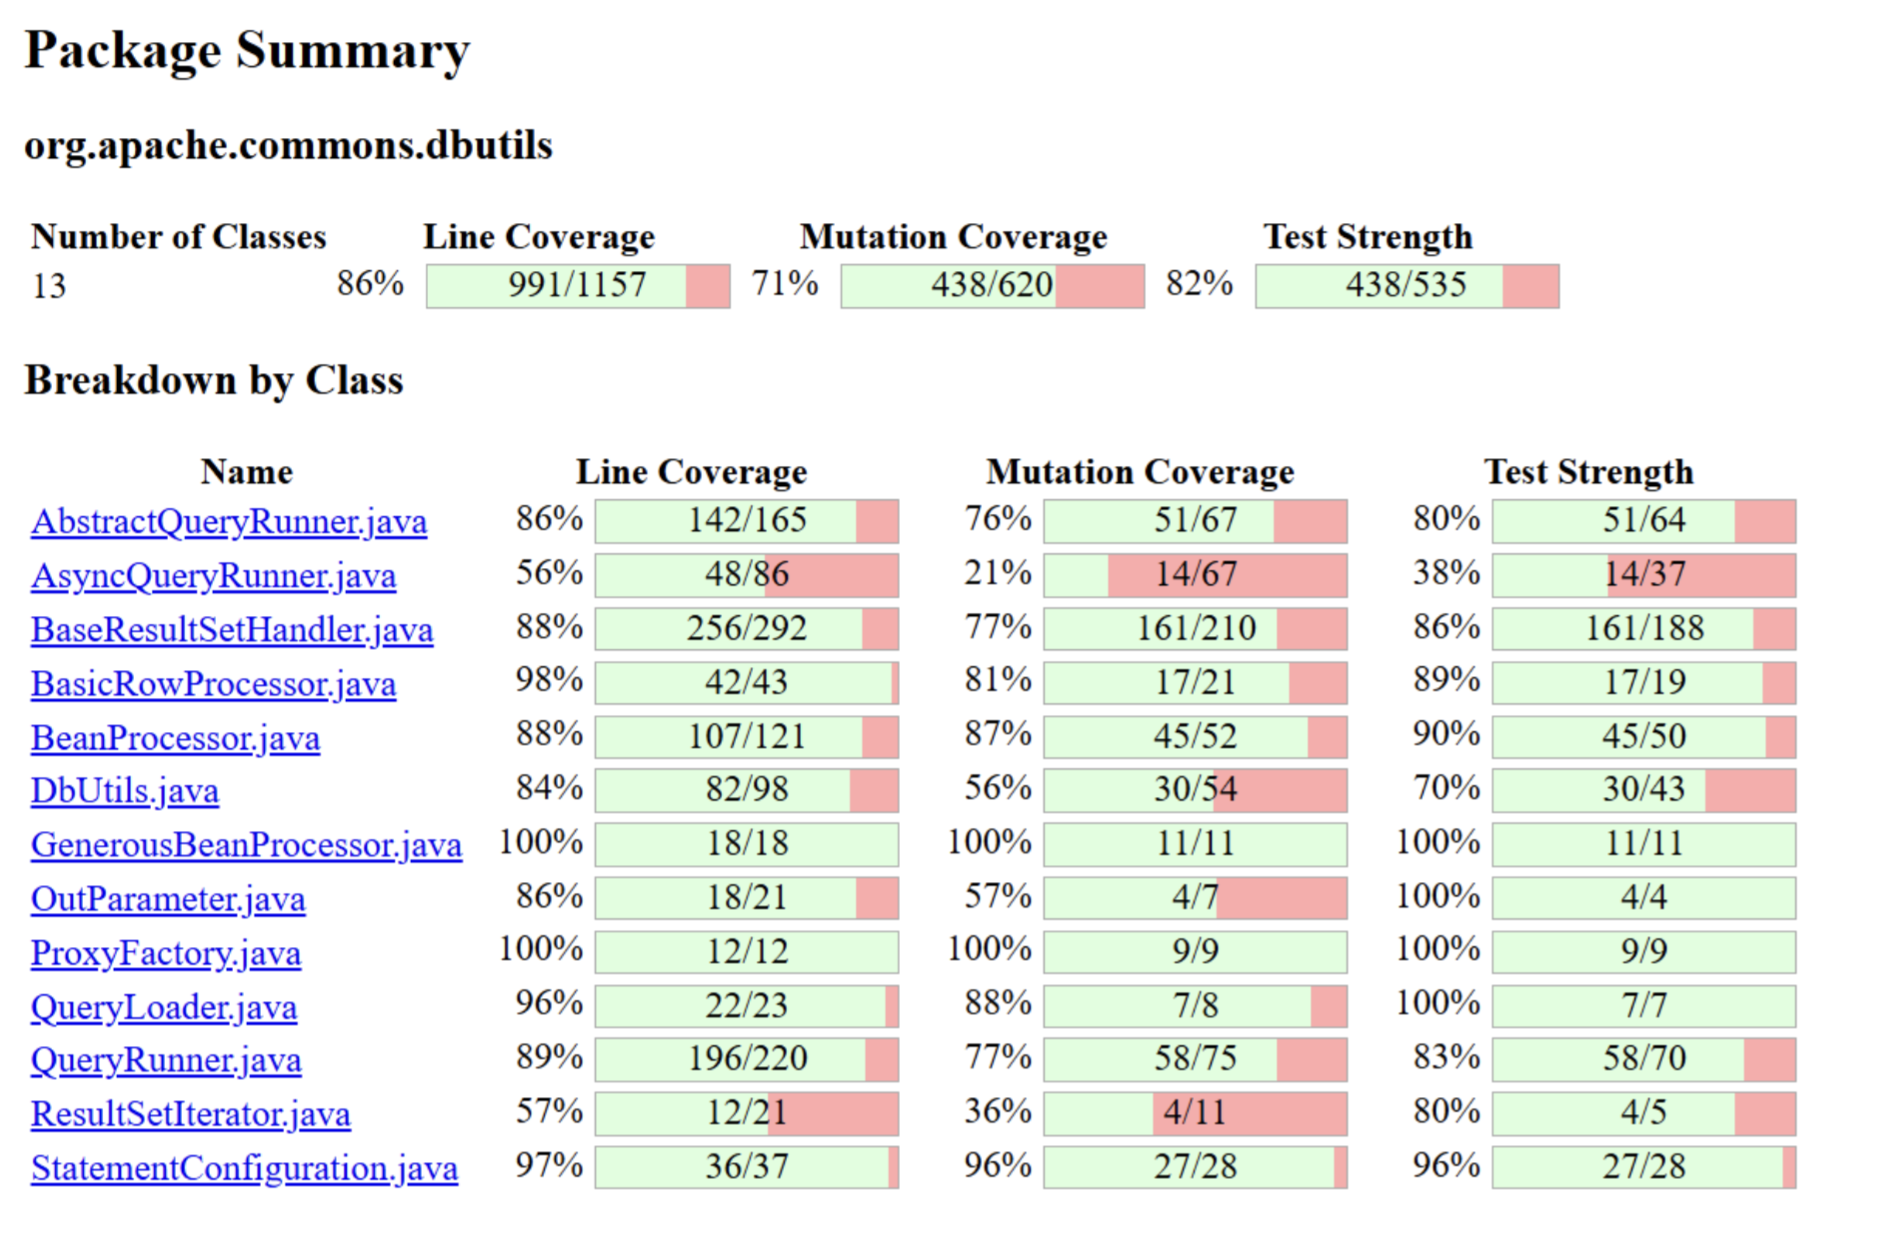
\includegraphics[width=1\linewidth]{images/pitest4.png}
    \caption{“org.apache.commons.dbutils” Package Pit Test Overview}
\end{figure}


Although the overall Mutation Coverage of this package improved significantly from 44\% to 71\%, and Test Strength saw a modest increase of 2 percentage points alongside a substantial rise in the number of tests, some classes still lack adequate mutation coverage and test strength. The test generation primarily targeted the classes \texttt{AsyncQueryRunner}, \texttt{DbUtils}, \texttt{QueryRunner}, \texttt{AbstractQueryRunner}, \texttt{BaseResultSetHandler}, and \\
\texttt{BeanProcessor}. While all six classes experienced notable improvements in both Mutation Coverage and Test Strength, there is still room for enhancement in \texttt{DbUtils} and \texttt{AsyncQueryRunner}. In particular, \texttt{AsyncQueryRunner} remains deficient in handling a significant number of mutations.

In future efforts, special attention should be given to these two classes to further strengthen the quality of their tests and address the existing gaps.

\section{Security analysis using OWASP FindSecBugs and OWASP DC.}

\subsection*{FindSecBugs}

All compiled classes of the project were analyzed with SpotBugs version 4.5.3 using the following command: 

\begin{lstlisting}
find-sec-bugs-version-1.13.0\cli\findsecbugs.sh -progress -html 
-output findSecBugsReport.html target\classes\org\apache\commons\dbutils
\end{lstlisting}

\begin{figure}[H]
    \centering
    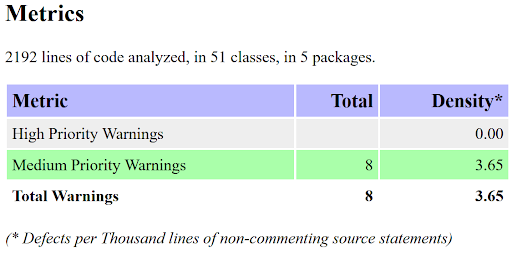
\includegraphics[width=1\linewidth]{images/owasp1.png}
    \caption{OWASP FindSecBugs results}
\end{figure}

Eight medium-priority warnings were found, all of them with the warning type “Security Warning.” One of them was about “possible information exposure through an error message” in the \texttt{DbUtils} class, while the other seven warnings were about possible weak points for SQL injections in both the \texttt{QueryRunner} and \texttt{AbstractQueryRunner} classes.

\begin{figure}[H]
    \centering
    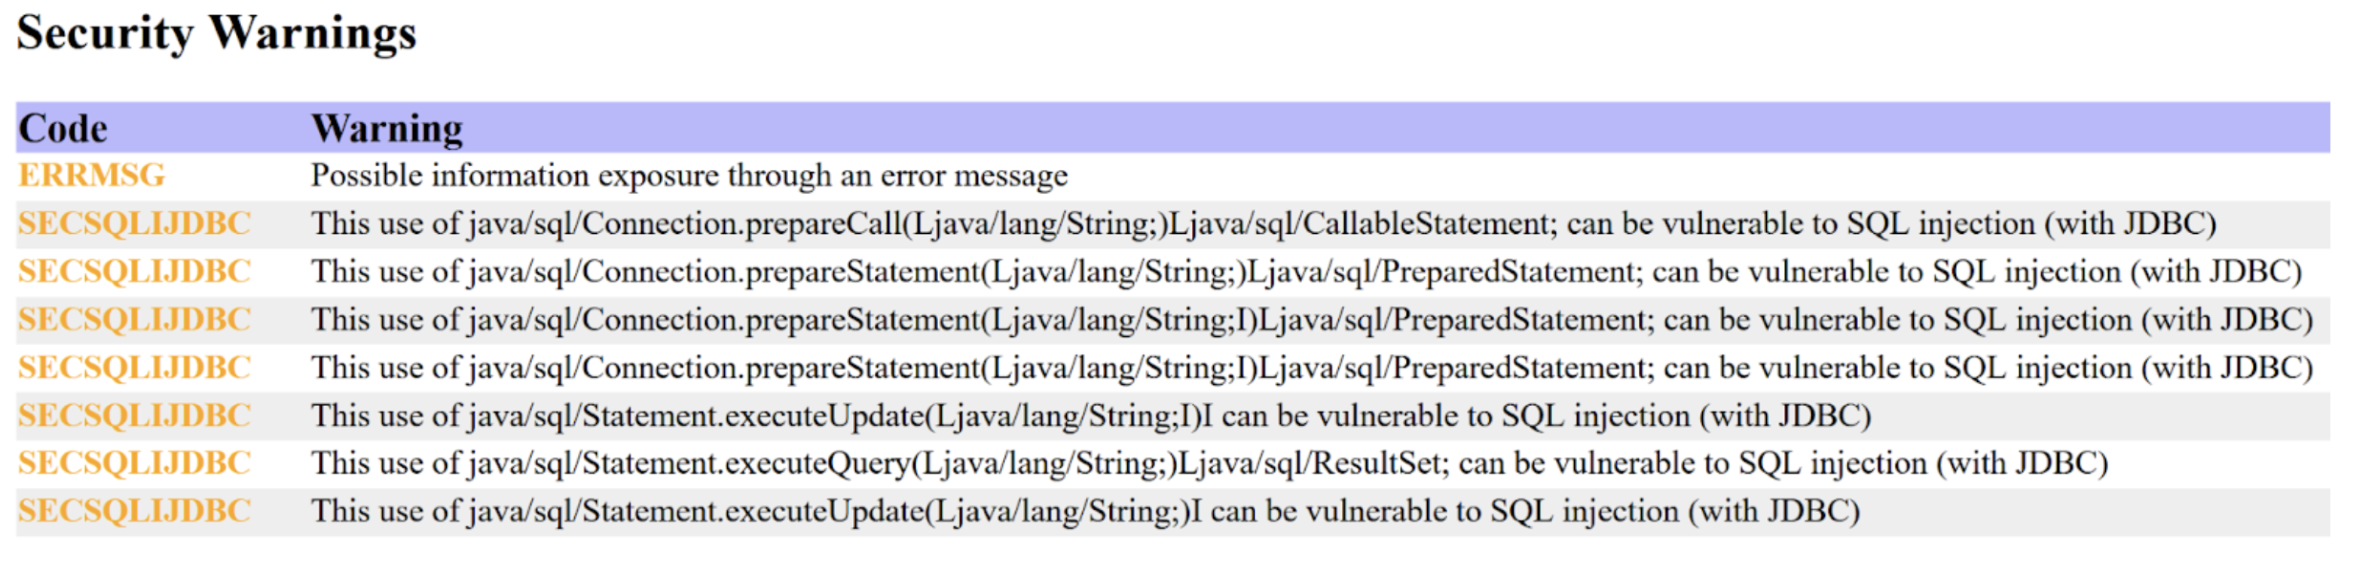
\includegraphics[width=1\linewidth]{images/owasp2.png}
    \caption{OWASP warnings list}
\end{figure}

\subsubsection*{\textbf{(Not) Addressing the Warnings}}

The information exposure warning was not addressed, as the line which caused the problem \\
(\texttt{next.printStackTrace(pw);}) is part of the \texttt{DbUtils} method \\
\texttt{printStackTrace}. As the purpose of this method is to print the stack trace, the warning can be seen as a false positive. Calling the method, on the other hand, could indeed present a risk of exposing too much information to the user, so it should be used with care.

In the \texttt{AbstractQueryRunner}, the factory methods \texttt{prepareCall} and two variations of \texttt{prepareStatement} use an SQL string as a parameter to create \texttt{CallableStatement} or \texttt{PreparedStatement}. As the SQL string is not checked, it was flagged as a potential threat. The methods mainly encapsulate the eponymous methods of the \texttt{java.sql.Connection} in a functional style and do not add security checks. The SQL string should not include the parameters yet but instead fill them later with the \texttt{fillStatement} method, also declared in the \texttt{AbstractQueryRunner} class. As the \texttt{apache.commons.dbutils} project is a library to be used in other projects, constructing the SQL statement securely lies with the developers of those projects. Therefore, nothing was changed in these methods.

The same applies to the \texttt{QueryRunner}'s \texttt{insert}, \texttt{query}, and \texttt{update} methods, which are the source of the other four warnings. They use the SQL string provided as a method parameter and insert the parameters into it if they were also provided as a method parameter. The method is only insecure if the caller chooses not to use the \texttt{params} parameter and constructs the SQL string beforehand in an insecure way.

\subsection*{Dependency Check}

With the given plugin for the dependency-check and the command:

\begin{verbatim}
mvn dependency-check:check
\end{verbatim}

the dependencies of the project were analyzed.

\begin{figure}[H]
    \centering
    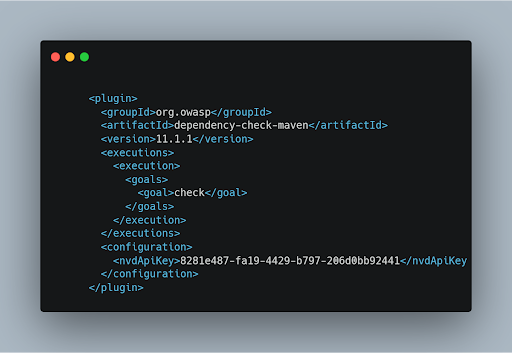
\includegraphics[width=1\linewidth]{images/owasp3.png}
    \caption{Dependency check}
\end{figure}

The dependency check found 0 vulnerabilities because the project does not have any dependencies outside of the test scope.

\end{document}